\documentclass{beamer}

\usetheme{kth}

\title[title]
{Predictive Safety Filter for Learning Controllers during Path Following}

% \subtitle
% {A Safety Guarantee for }

\author[Author] % (optional, use only with lots of authors)
{John~Liu\inst{1}} % \and S.~Another\inst{2}}

\institute[einride] % (optional, but mostly needed)
{
  \inst{1}%
  Einride Master's Thesis Program
}

\date[final presenation] % (optional, should be abbreviation of conference name)
{2022-06-16}

\footline{\today}

\AtBeginSubsection[]
{
  \begin{frame}<beamer>{Outline}
    \tableofcontents[currentsection,currentsubsection]
  \end{frame}
}
\begin{document}


\begin{frame}[plain, t]
  \titlepage
\end{frame}

\begin{frame}{Outline}
  \tableofcontents
\end{frame}

\section{Introduction}

\subsection{Research Problem}

\begin{frame}{Model-based Controllers}{Control Theory}
    \begin{itemize}
        \item Model-based controllers make assumptions about the vehicle
              dynamics and the external environment.
    \end{itemize}
\end{frame}

\begin{frame}{Learning Controllers}{Machine Learning}
    \begin{itemize}
        \item Learning controllers have a greater performance potential but
              lack safety guarantees.
    \end{itemize}
\end{frame}

\begin{frame}{Problem Formulation}
    \begin{itemize}
        \item Can a predictive safety filter ensure safety when it is not possible
              to fully model the real system dynamics? \pause
        \item Specifically, can predictive safety filter guarantee safety for the
              Einride pod during a path following task?
    \end{itemize}
\end{frame}

\section{Background}

\subsection{Vehicle Model}

\begin{frame}{Kinematic Model}
\end{frame}

\begin{frame}{Dynamic Model}
\end{frame}

\begin{frame}{Frenet Frame}{A coordinate system transformation}
    \begin{itemize}
        \item Path relative coordinate system.
    \end{itemize}
\end{frame}

\subsection{Gaussian Process Regression}

\subsection{Model Predictive Control}

\subsection{Predictive Safety Filter}

\subsection{The Basic Problem That We Studied}

\begin{frame}{Make Titles Informative. Use Uppercase Letters.}{Subtitles are optional.}
  \begin{itemize}
  \item
    Use \texttt{itemize} a lot.
  \item
    Use very short sentences or short phrases.
  \end{itemize}
\end{frame}

\begin{frame}{Make Titles Informative.}
  You can create overlays\dots
  \begin{itemize}
  \item using the \texttt{pause} command:
    \begin{itemize}
    \item
      First item.
      \pause
    \item
      Second item.
    \end{itemize}
  \item
    using overlay specifications:
    \begin{itemize}
    \item<3->
      First item.
    \item<4->
      Second item.
    \end{itemize}
  \item
    using the general \texttt{uncover} command:
    \begin{itemize}
      \uncover<5->{\item
        First item.}
      \uncover<6->{\item
        Second item.}
    \end{itemize}
  \end{itemize}
\end{frame}

\subsection{Previous Work}

\begin{frame}{Make Titles Informative.}
\end{frame}

\begin{frame}{Make Titles Informative.}
\end{frame}

\section{Results}

\subsection{Swing-up Pendulum}

\subsection{Vehicle Path Following}
\begin{frame}
    \begin{itemize}
        \item Unsafe system:
            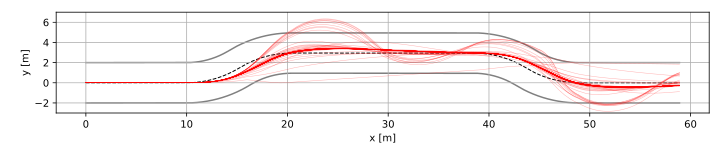
\includegraphics[width=0.9\textwidth]{figures/unsafe_200.pdf}
        \item Safe system:
            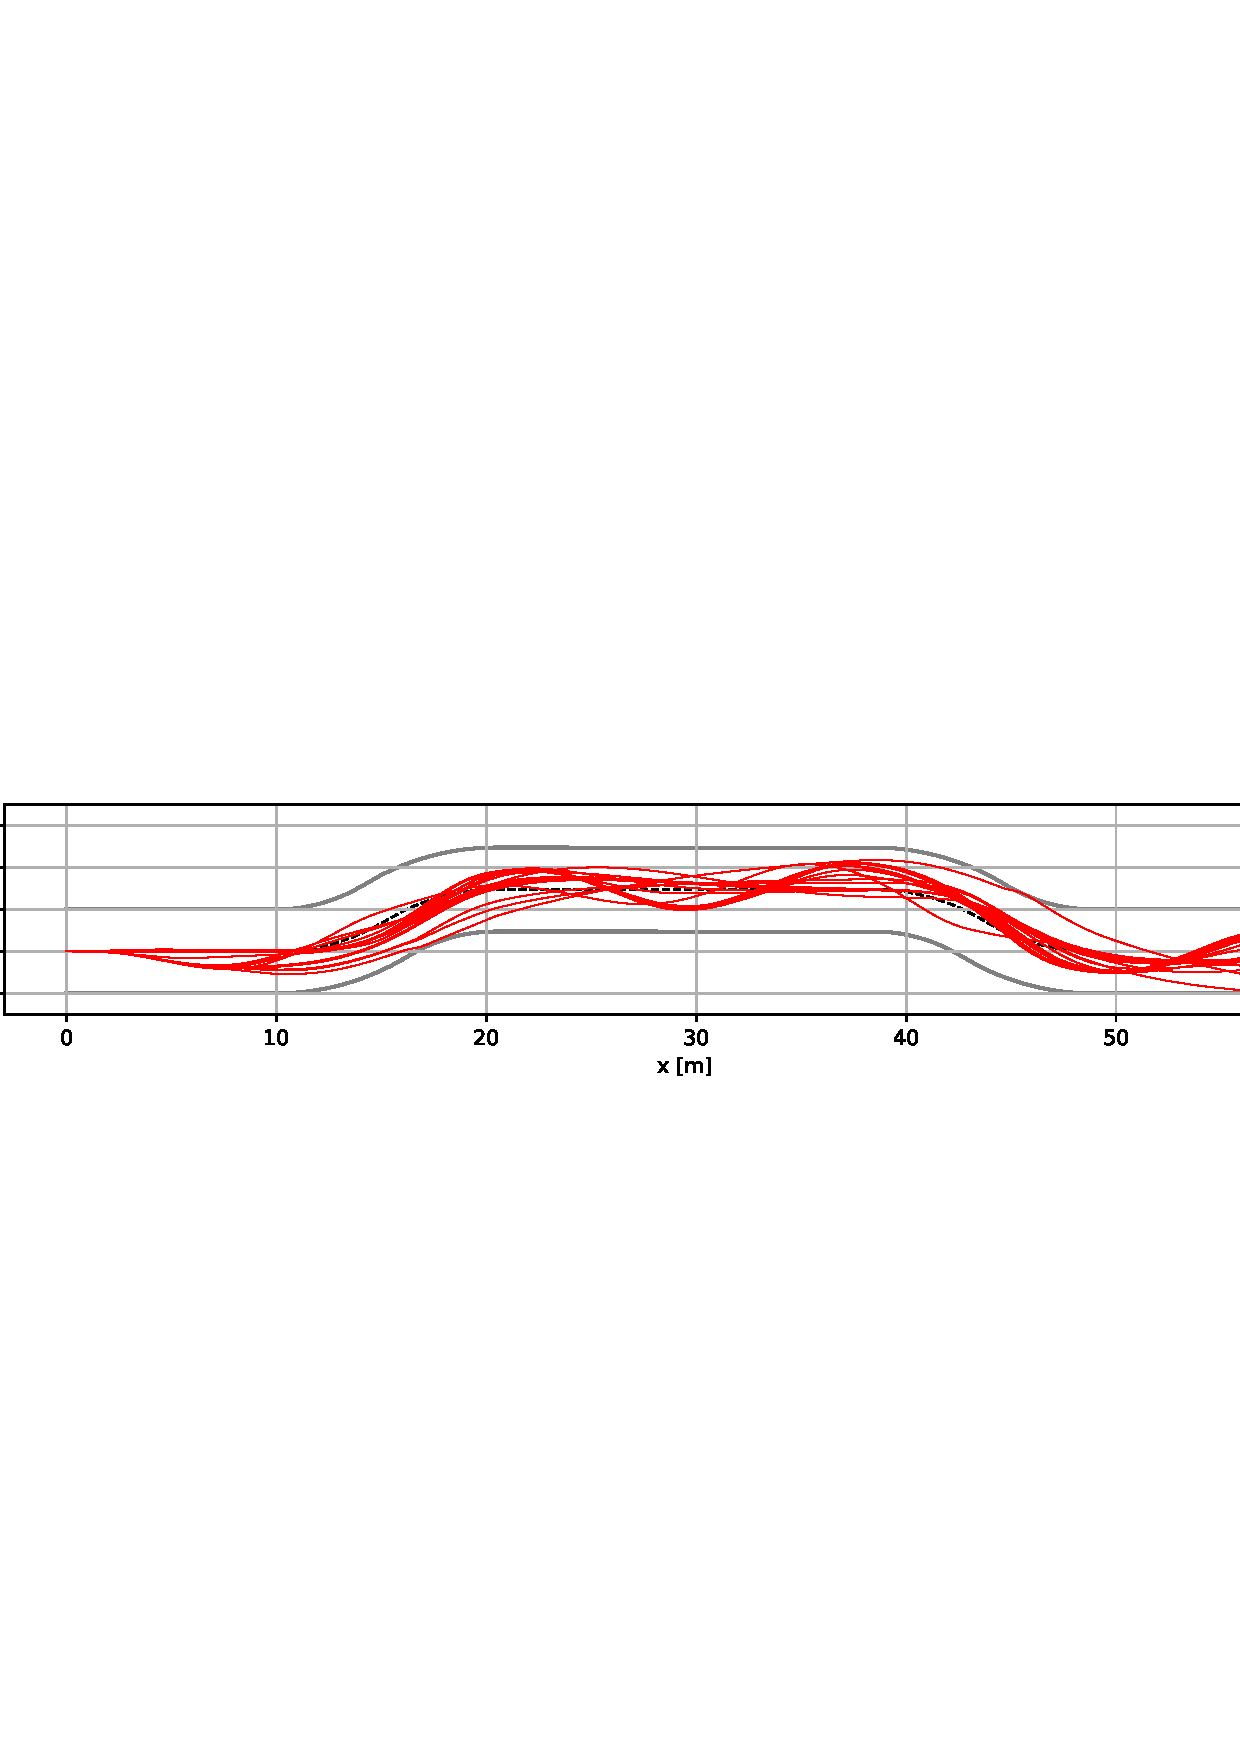
\includegraphics[width=0.9\textwidth]{figures/safe_200.pdf}
    \end{itemize}
\end{frame}

\subsection{Main Results}

\begin{frame}{Make Titles Informative.}
\end{frame}

\subsection{Basic Ideas for Proofs/Implementation}

\begin{frame}{Make Titles Informative.}
\end{frame}

\section*{Conclusion}

\begin{frame}{Summary}
  \begin{itemize}
  \item
    The \alert{first main message} of your talk in one or two lines.
  \item
    The \alert{second main message} of your talk in one or two lines.
  \item
    Perhaps a \alert{third message}, but not more than that.
  \end{itemize}

  \vskip0pt plus.5fill
  \begin{itemize}
  \item
    Outlook
    \begin{itemize}
    \item
      Something you haven't solved.
    \item
      Something else you haven't solved.
    \end{itemize}
  \end{itemize}
\end{frame}

\appendix
\section<presentation>*{\appendixname}
\subsection<presentation>*{For Further Reading}

\begin{frame}[allowframebreaks]
  \frametitle<presentation>{For Further Reading}

  \begin{thebibliography}{10}

  \beamertemplatebookbibitems

  \bibitem{Author1990}
    A.~Author.
    \newblock {\em Handbook of Everything}.
    \newblock Some Press, 1990.


  \beamertemplatearticlebibitems

  \bibitem{Someone2000}
    S.~Someone.
    \newblock On this and that.
    \newblock {\em Journal of This and That}, 2(1):50--100,
    2000.
  \end{thebibliography}
\end{frame}

\end{document}


